\documentclass[11pt,a4paper]{article}

\usepackage{geometry}
 \geometry{
 a4paper,
 total={150mm,237mm},
 left=30mm,
 top=30mm,
 }

% cf. http://tex.stackexchange.com/questions/50182/subtitle-with-the-maketitle-page
\usepackage{titling}
\newcommand{\subtitle}[1]{%
  \posttitle{%
    \par\end{center}
    \begin{center}\large\textbf{#1}\end{center}
    \vskip0.5em}%
}

\usepackage{color}
\usepackage{graphicx}
\usepackage[pdftex,colorlinks=false]{hyperref}
% get rid of the horrible coloured boxes around links
\hypersetup{
    colorlinks,%
    citecolor=black,%
    filecolor=black,%
    linkcolor=black,%
    urlcolor=black
}

\usepackage[utf8]{inputenc}
\usepackage[lf]{venturis} %% lf option gives lining figures as default; 
\usepackage[T1]{fontenc}
\usepackage{csquotes}
\usepackage[UKenglish,german]{babel}

\usepackage{fancyvrb}
\VerbatimFootnotes

\widowpenalty10000  % http://tex.stackexchange.com/questions/4152/how-do-i-prevent-widow-orphan-lines
\clubpenalty10000

\title{The SysSon Platform}
\subtitle{Technical Report TR-2016-08-1\\Institute of Electronic Music and Acoustics, Graz}
\author{Hanns Holger Rutz}
% \date{09-Feb-2016}
\date{August 2016}

% cf. https://tex.stackexchange.com/questions/94126/change-font-to-only-section-and-subsection-of-my-document
%\usepackage{titlesec}
%\titleformat{\chapter}[display]
%  {\fontfamily{pag}\selectfont\huge\bfseries}
%  {\chaptertitlename\ \thechapter}
%  {20pt}
%  {\Huge}
%\titleformat{\section}
%  {\fontfamily{pag}\selectfont\bfseries\Large}
%  {\thesection}
%  {1em}
%  {}
%\titleformat{\subsection}
%  {\fontfamily{pag}\selectfont\bfseries\Large}
%  {\thesection}
%  {1em}
%  {}

\usepackage[backend=biber,authordate]{biblatex-chicago} % citereset=chapter
%\usepackage[backend=biber,natbib,isbn=false,useprefix=true,sorting=ydnt]{biblatex-chicago} % citereset=chapter
% \addbibresource{all.bib} % add a bib-reference file
\addbibresource{rutz.bib} % add a bib-reference file

% warning: https://tex.stackexchange.com/questions/313477/
% \usepackage{csquotes}

\usepackage{tabularx}
% cf. https://tex.stackexchange.com/questions/84400/table-layout-with-tabularx-column-widths-502525
\newcolumntype{s}{>{\hsize=1cm}X}

% says you should load after babel and fontspec
\usepackage[shrink=10, babel=true]{microtype}	% http://tex.stackexchange.com/questions/141852/latex-allows-line-break-between-concluding-em-dash-and-comma-before-a-new-sub-cl/141854#141854

\newcommand{\todo}[1]{\colorbox{yellow}{\textsc{todo}: #1}}

\newcommand{\quot}[1]{\guillemotleft {#1}\guillemotright}

\newcommand{\worktitle}[1]{\textit{#1}}

\newcommand{\workentry}[2]{\vspace{7.5pt}\noindent\textbf{#1} (#2)}
\newcommand{\workentrySel}[2]{\vspace{7.5pt}\noindent\textbf{#1}$*$ (#2)}

\newcommand{\figref}[1]{Fig.~\ref{#1}}

\newcommand{\software}[1]{\textit{#1}}

\newcommand{\sysson}[0]{SysSon}
\newcommand{\syssonVersion}[0]{1.8.0}
\newcommand{\syssonVersionS}[0]{1.8.0-SNAPSHOT}

\begin{document}
% \begin{titlepage}
\maketitle
\selectlanguage{UKenglish}
\thispagestyle{empty}
\newpage
\section{\todo{}}

\subsection{Libraries and Modules}

\sysson{} is built with the \software{sbt} build tool.\footnote{\url{http://www.scala-sbt.org/}} \software{Sbt} manages module and library dependencies though a software called \software{Ivy} and using so-called \software{Maven} artefacts. Such artefacts are composed of a group-identifier, artefact-identifier, and a version string. For example, \sysson{} itself has group-id \verb!at.iem.sysson!, artefact-id \verb!sysson!, and current version \verb!1.8.0-SNAPSHOT!. The version scheme is the one proposed as \emph{Semantic Versioning}\footnote{\url{http://semver.org/}}, i.e. \verb!MAJOR.MINOR.PATCH!. The \verb!MAJOR! version indicates an entire new architecture, where the first stable generation is usually indicated by the digit \verb!1!. The \verb!MINOR! version indicates incremental changes, while the \verb!PATCH! version indicate bug fixes without change in functionality. In the Scala eco-system, the terminology is slightly different, where the major version is called "epoch", the minor version is called major version and the patch version is called minor version. So Scala 2.11.8, the latest release, has epoch 2, major version 11, and minor version 8 in the Scala terminology. We will henceforth use this naming scheme. The special suffix \verb!-SNAPSHOT! indicates that the version is not a stable released artefact but work in progress. Stable artefacts of libraries are published to a repository such a the public Maven Central,\footnote{\url{http://central.sonatype.org/}} and build tools can thus automatically download required artefacts based on a description of an application's dependencies.

The Maven based build tool \software{sbt} assumes a \emph{binary compatibility} between all minor versions, whereas the major version must be incremented when a binary incompatible change is introduced. A binary incompatibility means that the Java byte code of the library contains changes that make it unsafe for use with a caller that was compiled against a different version. This happens for example if a method has been removed from public API or changed in signature. Sbt automatically chooses the highest minor version if there are several transitive dependencies on the same artefact but with different minor versions, while it warns when transitive dependencies exist for the same artefact with different major versions. This also applies to the Scala version a library was compiled against, meaning that a binary file resulting from compilation against Scala 2.10.x (where x is any minor version) is binary incompatible with a binary file resulting from compilation against Scala 2.11.x (with 2.11.8 being the currently most recent release version). To ease this difficulty, sbt has introduced a mechanism called cross-versioning. Often Scala releases are still source compatible, and thus it is possible, for example, to compile the same source code against Scala 2.10.x and 2.11.x without changes. The artefacts will then be ``tagged'' by appending the major Scala version, e.g. the artifact-id becomes \verb!sysson_2.11! when compiling against Scala 2.11.x (this is independent of the regular Maven version).

This versioning scheme can be observed in the dependency graph that shows all the libraries and transitive libraries,\footnote{Transitive means a library A is used by another library B, and B is used by \sysson{}. Then A is a transitive dependency of \sysson{}.} generated by the \software{sbt-dependency-graph} plugin\footnote{The call is \verb!sbt dependencyDot!.} and shown in \figref{fig:dependencies}.\footnote{In the figure, lower level transitive third-party dependencies have been omitted for a clearer overview.} We can see the \sysson{} main artefact on the left-hand side with arrows pointing to immediate dependencies (libraries), which in turn point to other transitive libraries. Some libraries are published as a set of related artefacts, often bound together by one ``virtual'' meta-package. For example, the \software{Mellite} computer music environment is actually composed of two artefacts \verb!mellite-core! and \verb!mellite-views!, combined as virtual artefact \verb!mellite!. The \verb!-views! artefact connects to the graphical user interface, whereas \verb!-core! only contains data structures. Since \verb!-views! depends on \verb!-core! but not vice versa, it means we can develop a library merely based on the data structures without requiring the dependency on any GUI.

\subsubsection{Licensing Questions}

This approach helps keeping the code base modular, and furthermore can improve the licensing situation: In general we try to avoid dependency on GPL licensed code,\footnote{\url{https://www.gnu.org/licenses/gpl.html}} because it enforces the GPL on the entire product, something that is not the case with the LGPL\footnote{\url{https://www.gnu.org/copyleft/lesser.html}} or even more permissive licenses. We try to decouple GPL dependencies as far as possible, allowing for LGPL terms in most cases. GPL artefacts are often commercially developed products, because a commercial client company will likely not want to release their own product as open source under GPL terms and is thus forced to buy a commercial license from the library vendor, an approach that is called dual licensing. For example, the \software{iText} PDF library is available for free under GPL terms or by buying a commercial license that allows the client to develop their product without requiring to open source it. The same is true for the \software{Berkeley DB} database (developed by Oracle) and the \software{WebLaF} user interface look-and-feel. We currently do not own any commercially bought licenses, and thus \textbf{\sysson{} must be licensed under GPL version 3} terms. However except for the mentioned GPL based libraries, we have control over most other libraries, and thus in the future a different license might be chosen if replacements are found for the GPL libraries (or commercial licenses purchased).

\begin{figure}%
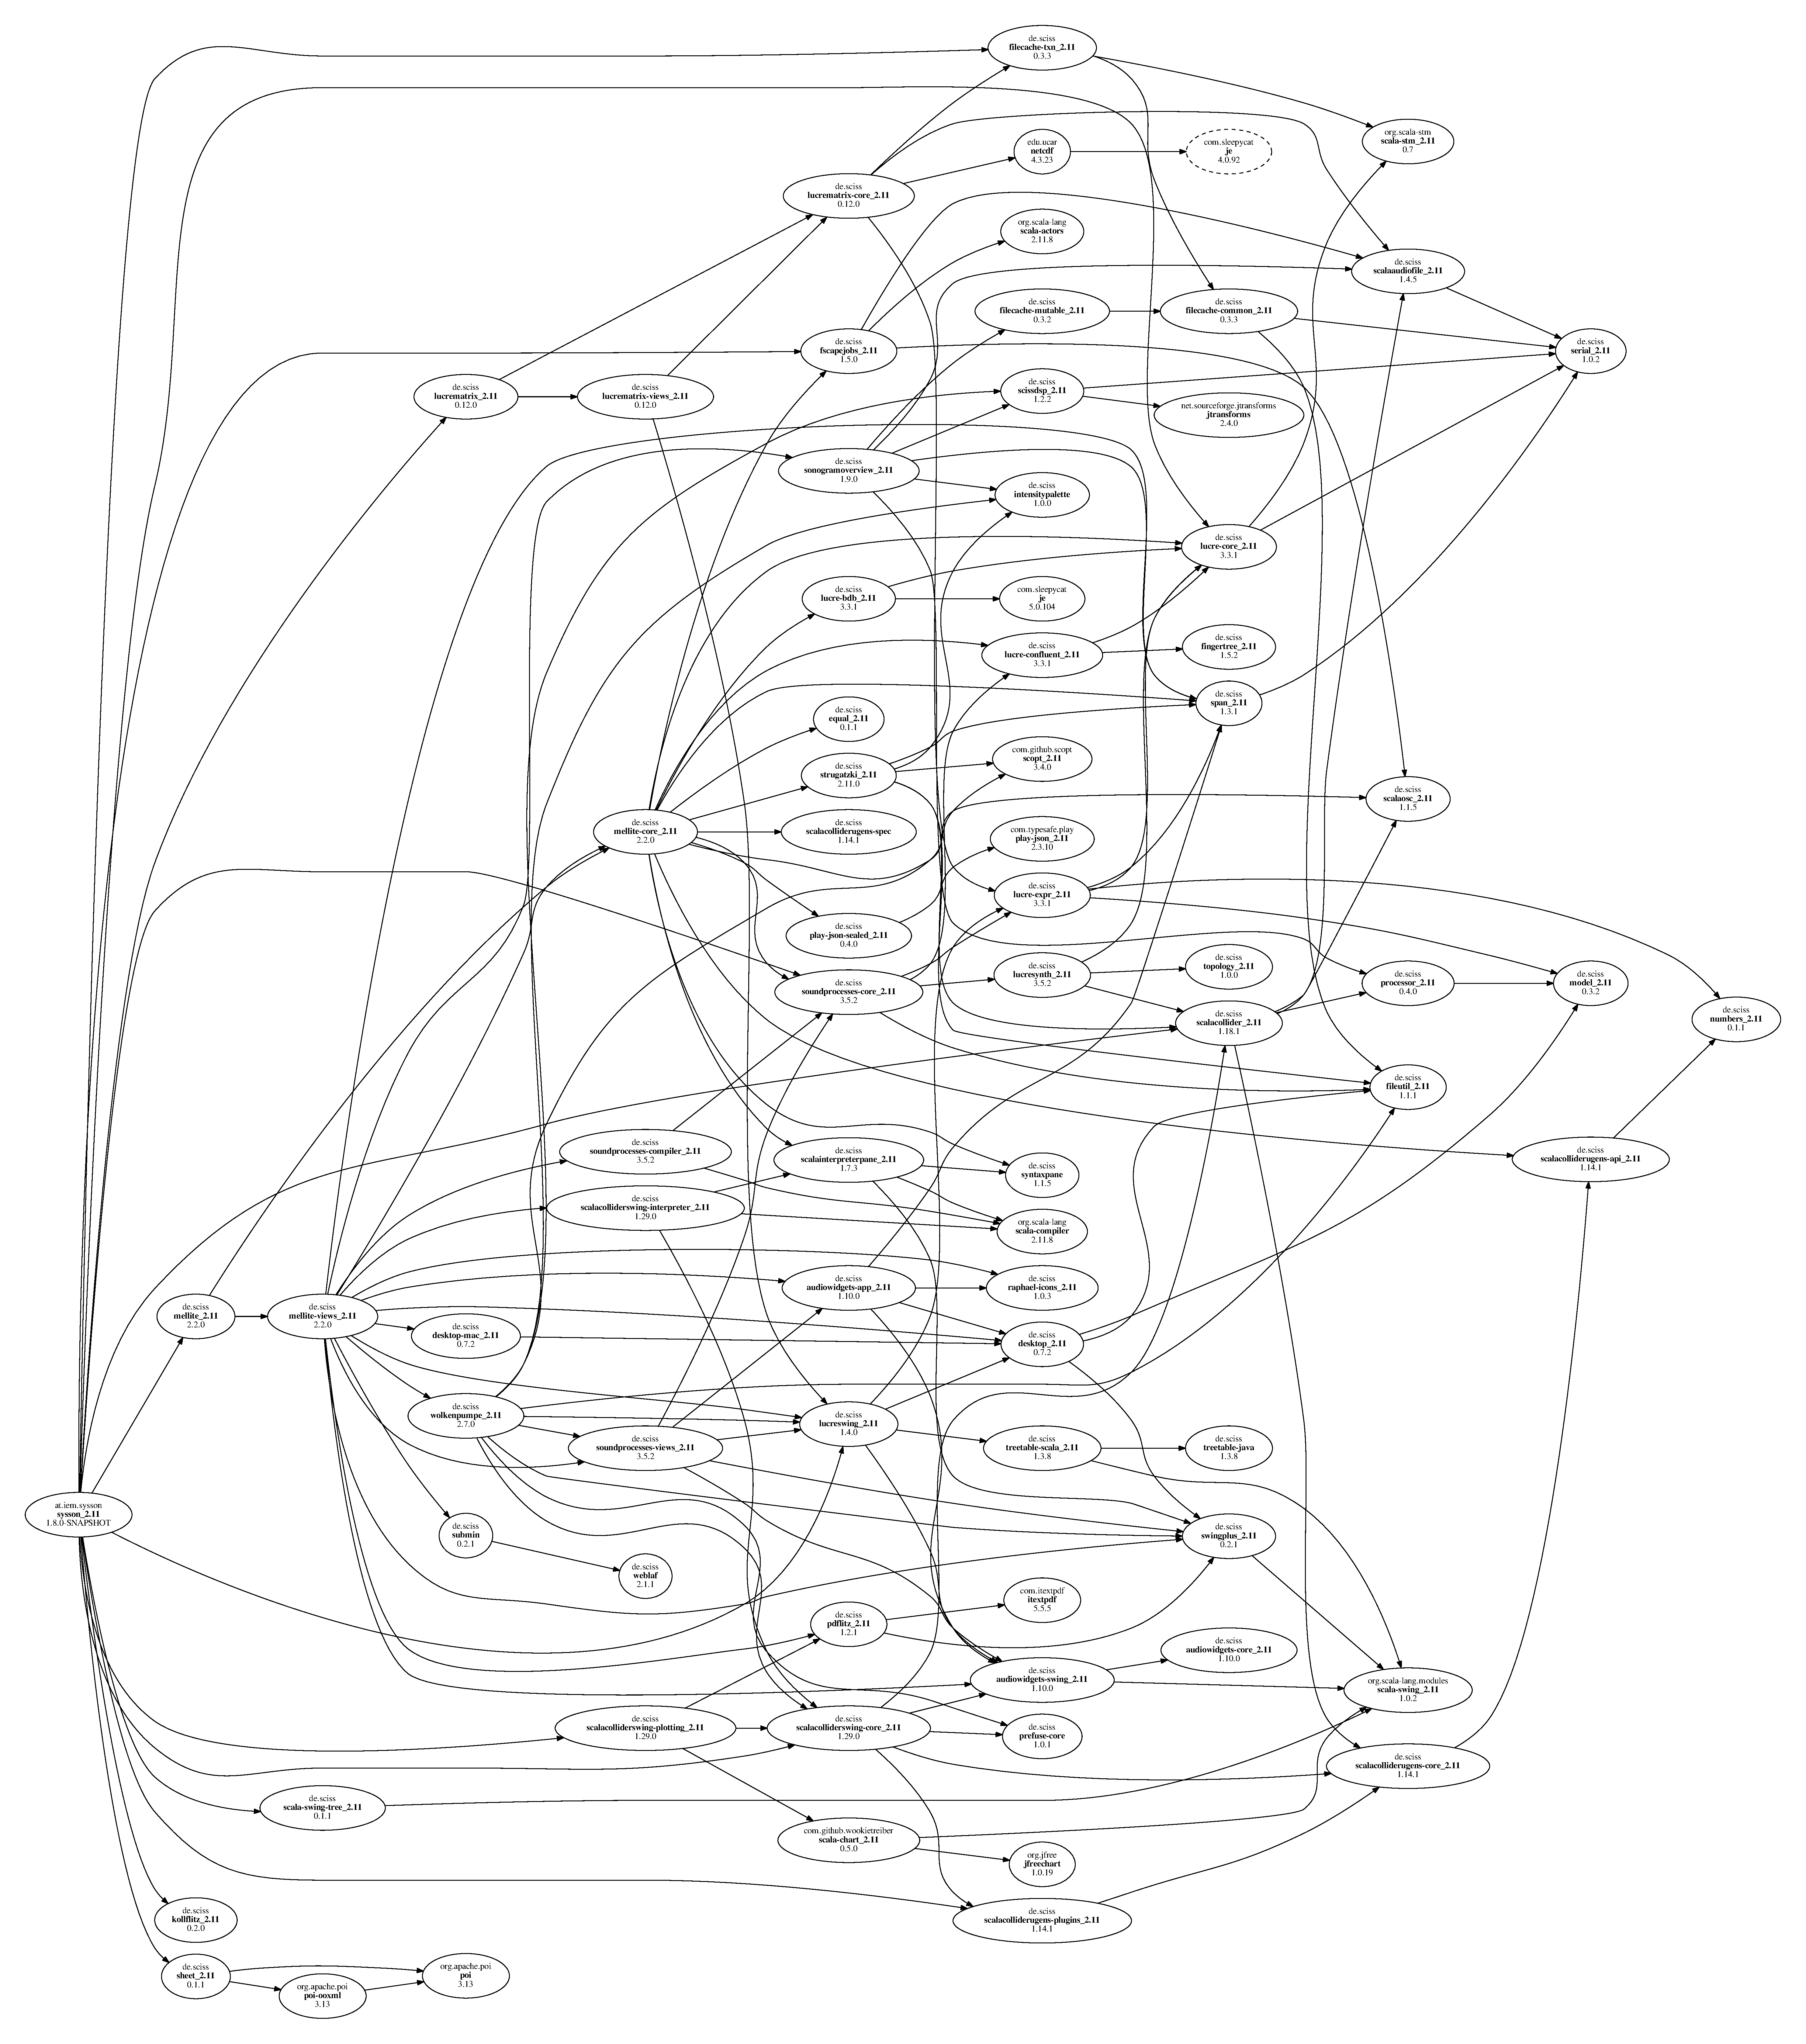
\includegraphics[width=\textwidth,trim=15mm 15mm 15mm 15mm]{figures/dependencies-compile.pdf}%
\caption{Module/library dependencies for SysSon version \syssonVersion{}}%
\label{fig:dependencies}%
\end{figure}

\subsubsection{Description of Modules}

We will now give a brief overview of the modules and libraries on which \sysson{} relies and which were shown in \figref{fig:dependencies}.

\paragraph{Mellite}

By far the strongest dependency is on the \software{Mellite} computer music environment. In fact, \sysson{} can be understood as a domain specific extension of \software{Mellite}, adding abstractions for sonification and matrix data, although the GUI is also slightly different.
%
Mellite is a graphical front end and application built on top of the \software{SoundProcesses} library. It introduces a tree based workspace structure with graphical views and editors for various objects.

\textbf{Artefacts:} \verb!-core! contains objects in addition to \software{SoundProcesses}, such a color, the workspace and cursors abstractions, and a set of editing operations. \verb!-views! contains the graphical user interface, and undo-redo editing facilities.

\textbf{Assessment:} The workspace abstraction should probably be moved directly into the \software{SoundProcesses} project, making the \verb!-core! artefact superfluous. It could be useful to define public API in a separate \verb!-api! artefact and create sub-modules for specific editors that do not necessarily have to be bundled in every application. An example is the \software{Wolkenpumpe} live improvisation tool that is currently a dependency of \verb!-views!.
A big challenge is the inter-linkage between visual representations and text-based editing. While the model-view approach already makes programmatic changes instantly visible across the UI, there is no global UI protocol through which the views ``know each other'' such that for example selecting one view implies a visual highlight on related views. Also because of the traditional windowing system, there are challenges in connecting objects (e.g. through ``cords'') across different windows. A radical revision of \software{Mellite} could focus on making text-editing a first class citizen, e.g. by allowing to activate a text-based view for every object on the UI. In terms of \sysson{}, an interesting model to look at might be the ``notebook'' approaches taken with software such as Jupyter.\footnote{\url{http://jupyter.org/}}

\paragraph{Lucre-Matrix}

Defined as a separate library, this module provides a matrix data abstraction, bridging \software{NetCDF} and the transactional-memory model defined by \software{Lucre} and underlying \software{SoundProcesses}. It makes it possible to build data-flow graphs, e.g. by applying a dimensional reduction operation to an input matrix, yielding a graph that constitutes a new compound matrix object.

\textbf{Artefacts:} \verb!-core! contains the data structures, and a mechanism for caching matrix data in sound files (\sysson{}'s way of passing matrix data to \software{ScalaCollider}). \verb!-views! contains the graphical user interface element, noticeable as the matrix editor component in \sysson{}'s sonification editor.

\textbf{Assessment:} The number of operations that can be performed on the matrices is quite small. It would also be worth exploring the possibilities of using a different matrix abstraction than the one of \software{NetCDF} as blue print, linking this library closer with standard ``data science'' frameworks. Another huge question arises from the way sonification models are built in \sysson{}. It appears that it may become much more important to be able to pre-process matrix data before they become part of the real-time sound synthesis. One way to conceive this is through additional ``graph elements'' in the sonification synthesis definition, i.e. as is done with elements such as \verb!Dim#values!. The down-side of this is that we risk duplicating the functionality on the ``Lucre side'' vs. the ``ScalaCollider side''. Therefore, the development of \software{Lucre-Matrix} very much depends on the evolution of the sonification model in \sysson{} and the way in which one will be able to represent ``sonification programs'', the way in which these programs can be ``co-edited'' with synthesis definitions.

\paragraph{Lucre}

The name \software{Lucre} serves as a placeholder for an approach to memory and data modelling based on software transactional memory (STM). \software{Lucre} defines an abstract system layer that usually occurs in objects as a type parameter \verb!S!, e.g. \verb!Sonification[S]!. At runtime, different systems can be initiated: an ephemeral pure in-memory system, a durable system where objects are automatically persisted to hard-disk, and a confluent system which extends the durable system with a version history of the modification of objects. This kind of temporal database approach has been developed extensively through my thesis \autocite{rutz2014tracing}, and forms the basis for \software{SoundProcesses}, \software{Mellite}, and \sysson{} respectively.

\textbf{Artefacts:} There is currently no umbrella meta package. \verb!-core! is now a rather comprehensive artefact that includes four packages \verb!stm!, \verb!geom!, \verb!data!, \verb!event!. The reactive event propagation mechanism is now baked into the fundamental \verb!stm! package (this was not the case with older versions). This package defines the basic types \verb!Sys! (memory-model abstraction), \verb!Txn! (transaction), \verb!Cursor! (transaction initiator), \verb!Elem! (an element that publishes events and that can be copied), and \verb!Obj! (an element that in addition to \verb!Elem! has a unique identifier and an attribute map). Most data types in \sysson{} and and \software{SoundProcesses} inherit from \verb!Obj!. The \verb!event! package defines the infrastructure for event dispatch (publisher-subscriber mechanism). The \verb!data! package contains several data structures needed for the implementation of various systems, e.g. lists, trees, spatial search structures. The second artefact is \verb!-expr! that introduces reactive expressions, with implementations for primitive types such as strings, boolean values, integer and floating point numbers, time spans (a pair of 64-bit integers), collections---\verb!BiPin! for a ``flat'' sequence or breakpoint function, \verb!BiGroup! for a sequence with possibly overlapping elements---and \verb!Artifact! (file object). While in-memory and ephemeral-durable systems are defined in the base package, actual database back-ends are defined by \verb!-bdb! and \verb!-bdb6!, both using the \software{Berkeley DB Java Edition} (BDB DB JE), introducing the dependency on the GNU GPL. \verb!-bdb! uses version 5, compatible with the JVM version 6, and \verb!-bdb6! uses version 6, requiring JVM version 8. The \verb!-confluent! artefact implements the confluently-persistent (versioned) system.

\textbf{Assessment:} Changes in \software{Lucre} fundamentally affect all parts of \sysson{}, as it is a deep dependency that is used by \software{SoundProcesses}, \software{Mellite}, \software{Lucre-Matrix} and others. The current version is stable and reliable but has a number of shortcomings: On the programming level, the syntactic overhead of carrying around system type parameter \verb!S <: Sys[S]]! as well as transaction context method argument \verb!implicit tx: S#Tx! is high, making it a rather bad fit for a light-weight domain specific language to define snippets in \software{Mellite} or \sysson{}. In the medium term future, this might be alleviated by the next generation Scala language (Dotty research project), where on the one hand type projections are seriously constrained, probably making it necessary to redefine the way system abstraction is visible in \software{Lucre}, but on the other hand also allowing to ``hide'' type parameters as type members and implicit arguments as implicit capabilities of a function's return type. However, this is a perspective of several years into the future, so in the shorter term, probably the most convincing solution is to add a separate DSL layer where transactional semantics are injected into the interpreter's code execution. Another question concerns the cost of \verb!Obj! instances. In previous versions we distinguished between expressions and these objects, making it for example possible to have cheap constant values. Constants appear very frequent, for example if one edits a numeric value in \sysson{} through a slider, many new objects have to be created (and persisted to the database) for each intermediary state in the dragging operation. With \verb!Obj! being basically the atoms for most operations, this means that now we have to allocate a lot of throw-away object identifiers and the space usage in the database is much higher than with the old ``simple'' constants, where only the containing \verb!S#Var! variable (mutable placeholder) was requiring a one-time allocation. It is thus desirable to rethink this atomicity and try to combine the simplicity of one layer \verb!Obj!-everywhere with the performance of having cheap constants. Somehow related to this is the lack of any sort of automatic garbage collection for transitory values. If we had a reference counting ability, we could evict objects from the database once they are not reachable any longer, or those transitorily produced during a transaction without having an actual linkage to the workspace at the commit-time of the transaction. A reference tracking could also help with automatically detecting ``bottom-up'' dependencies between objects in the GUI. Furthermore, we need to assess the necessity for the full confluent persistence in versioning---while theoretically elegant, we cannot abstract over the meld operation in the system layer, because there is no equivalent for ephemeral systems. Therefore, we are forced to introduce a object-copying mechanism agnostic of the system capabilities. Also, confluent meld could become expensive if used excessively, as the version paths grow linearly with the levels of meld. It might thus be more pragmatic to simplify the versioning system by moving to the less powerful partial persistence and improving on the definition of object-copying. Object-copying could also preserve information about the source object from which a copy was made, as this information is currently lost and thus undermines the effort to version objects. Another problem is the size of transactions. Transactions can become quite large which poses a problem for the database commit phase, as ACID requires that we wait for the durability guarantee at the end of each transaction. There is a ticket\footnote{\url{https://github.com/Sciss/Lucre/issues/6}} to evaluate other database back-ends, something that will also interact with the \software{Serial} module. It seems that especially in concurrent situations with conflicting transactions, we face performance problems or even impasses where the database times out. Going away from STM as the memory model would however require an entire new architecture, and so far STM has proven a very robust approach, so it is probably advisable to stay with it for the time being, instead evaluating strategies to undo the bottle-necks with concurrent transactions.

So far we have used BDB DB JE 5 to allow \sysson{} to run on legacy computers with Java 6, such as Mac OS X 10.6. The next version of \sysson{} can probably drop that constraint and require presence of Java 8 and thus the newer database version.

\paragraph{Lucre-Swing}

Published as a separate library, this module provides a set of simple widgets that can interface with expressions and other data structures from the \software{Lucre} project.

\paragraph{Serial}

This module defines a small serialization layer used by \software{Lucre} and other libraries.

\textbf{Assessment:} The module is optimised for speed and size, making serialization quite efficient. However, a current drawback is vulnerability to schema evolution. Serialised objects simply become unreadable if the schema is altered without any precautions in place that can parse older versions. In many cases it may simply not be possible to parse older versions, and in those cases it would be required to entirely ``upgrade'' an objects, for example allocating additional objects. While such upgrades are currently not foreseen, there are also made nearly impossible by the fact that the same entity might be written multiple times in the database. If every \verb!Obj! with an identifier \verb!S#ID! would be written as a small reference to one and the same location in the database, perhaps upgrading schemas would become feasible. For robustness, it would also be very helpful if an automatic export to other formats such as JSON would be available. This would require the serialisation API to change, for example including field names. Another current limitation is the prohibition of reference cycles within the same serialisation, something that can currently be worked around by the indirection of a \verb!S#Var!. Finally, one must currently write serialisers by hand which from our experience is \emph{very} prone to errors, and also clutters the source code unnecessarily. After deciding on an updated API, it might thus be advisable to look into macro-based synthesis of serialisers.

\todo{continue here}

\printbibliography

\end{document}
